\documentclass[10pt,a4paper]{article}

\usepackage[a4paper,top=0.85cm,bottom=0.85cm,left=1.05cm,right=1.05cm]{geometry}
\usepackage{fontspec}
\usepackage[french]{babel}
\usepackage[hidelinks]{hyperref}
\usepackage{xcolor}
\usepackage{graphicx}
\usepackage{titlesec}
\usepackage{enumitem}

\setmainfont{Arial}
\pagestyle{empty}
\setlength{\parindent}{0pt}
\setlength{\parskip}{0pt}
\linespread{0.96}
\hyphenpenalty=10000
\exhyphenpenalty=10000
\sloppy
\setlist[itemize]{leftmargin=1.05em,itemsep=0pt,topsep=1pt,parsep=0pt,label=-}
\urlstyle{same}

\definecolor{heading}{HTML}{123867}
\titleformat{\section}{\large\bfseries\color{heading}}{}{0pt}{}[\vspace{-5pt}\rule{\linewidth}{0.5pt}]
\titlespacing{\section}{0pt}{5pt}{3pt}

\newif\ifwithphoto
\withphotofalse
\IfFileExists{with_photo.flag}{\withphototrue}{}

\newcommand{\role}[3]{%
  \textbf{#1} \hfill #3\\
  \textit{#2}\vspace{1pt}
}

\newcommand{\edu}[4]{%
  \textbf{#1} -- #2 \hfill #3 #4\\[-1pt]
}

\begin{document}

\ifwithphoto
\begin{minipage}[c]{0.76\linewidth}
{\LARGE \textbf{Kossi Richard Allado}}\\
\textbf{Étudiant ingénieur en cybersécurité et IA | Pentest, sécurité web, offensive security}\\
Beni Mellal, Maroc | +212 621 074 305 | \href{mailto:alladokossirichard2025@gmail.com}{alladokossirichard2025@gmail.com}\\
\href{https://allakori.github.io/}{allakori.github.io} | \href{https://github.com/ALLAKORI}{github.com/ALLAKORI} | \href{https://www.linkedin.com/in/kossi-richard-allado-50177b2a5}{linkedin.com/in/kossi-richard-allado}
\end{minipage}
\hfill
\begin{minipage}[c]{0.18\linewidth}
\raggedleft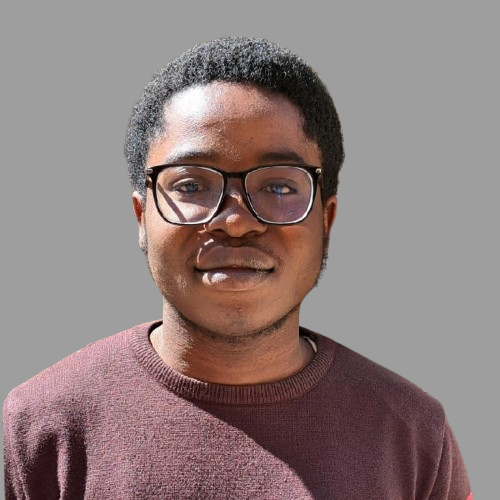
\includegraphics[width=2.35cm]{photo_richard.png}
\end{minipage}
\else
{\LARGE \textbf{Kossi Richard Allado}}\\
\textbf{Étudiant ingénieur en cybersécurité et IA | Pentest, sécurité web, offensive security}\\
Beni Mellal, Maroc | +212 621 074 305 | \href{mailto:alladokossirichard2025@gmail.com}{alladokossirichard2025@gmail.com}\\
\href{https://allakori.github.io/}{allakori.github.io} | \href{https://github.com/ALLAKORI}{github.com/ALLAKORI} | \href{https://www.linkedin.com/in/kossi-richard-allado-50177b2a5}{linkedin.com/in/kossi-richard-allado}
\fi

\section{Profil}
Étudiant ingénieur en cybersécurité et IA à l'ENSA Beni Mellal, orienté pentest junior, sécurité web, reconnaissance et exploitation encadrée. Portfolio GitHub avec CTF, labs DVWA SQL injection/XSS, Linux security, IAM/PKI et write-ups techniques. Recherche un stage PFA à partir de juillet 2026 en pentest, sécurité applicative, audit web ou offensive security junior.

\section{Compétences techniques}
\textbf{Pentest / web security :} Kali Linux, Burp Suite, Nmap, Wireshark, Hydra, reconnaissance, SQL injection, XSS, DVWA.\\
\textbf{Méthodologie offensive :} énumération, exploitation web, analyse de vulnérabilités, preuves, write-ups, remédiation.\\
\textbf{Systèmes / IAM :} Linux, SSH, SELinux, AppArmor, Lynis, Keycloak, MFA/TOTP, RBAC, OpenSSL, PKI.\\
\textbf{Programmation :} Python, Bash, C, SQL, Git/GitHub, Pandas, Scikit-learn, Jupyter.

\section{Projets techniques}
\textbf{CSIA CTF 2026 - 1ère place avec Team GHOSTSHELL} \hfill 2026\\
\href{https://github.com/ALLAKORI/csia-ctf-2026-writeups}{github.com/ALLAKORI/csia-ctf-2026-writeups}
\begin{itemize}
  \item Résolu en équipe des challenges web, OSINT, forensic, stéganographie et misc sous contrainte de temps.
  \item Rédigé des write-ups reproductibles avec hypothèses, commandes, preuves et raisonnement de résolution.
\end{itemize}

\textbf{Sécurité web, IAM et PKI} \hfill 2025\\
\href{https://github.com/ALLAKORI/cybersecurity-iam-labs}{github.com/ALLAKORI/cybersecurity-iam-labs}
\begin{itemize}
  \item Testé des vulnérabilités applicatives sur DVWA : SQL injection, XSS, analyse des causes et contre-mesures.
  \item Déployé un laboratoire Keycloak/OpenSSL : utilisateurs, rôles, MFA/TOTP, RBAC, PKI et contrôle d'accès.
\end{itemize}

\textbf{Investigation Volt Typhoon : compréhension du chemin d'attaque} \hfill 2026\\
\href{https://allakori.github.io/writeups/tryhackme/volt-typhoon/}{allakori.github.io/writeups/tryhackme/volt-typhoon}
\begin{itemize}
  \item Reconstruit une intrusion APT sur 9 phases MITRE ATT\&CK avec abus de WMIC, PowerShell, certutil, netsh et Mimikatz.
  \item Extrait 10+ indicateurs exploitables : compte compromis, IP source, web shell, staging directory, C2 et journaux effacés.
\end{itemize}

\textbf{Linux Security Labs : hardening et audit système} \hfill 2026\\
\href{https://github.com/ALLAKORI/linux-security-labs}{github.com/ALLAKORI/linux-security-labs}
\begin{itemize}
  \item Documenté un workflow Linux couvrant hardening, auditd, détection, artefacts système et analyse mémoire.
  \item Corrélé processus, connexions réseau et traces utilisateur pour produire un rapport orienté remédiation.
\end{itemize}

\section{Expérience}
\role{Stagiaire IA / Maintenance prédictive}{ONEE - Branche Eau, Kasba Tadla}{Août 2025}
\begin{itemize}
  \item Préparé des données capteurs de pompe haute pression et entraîné un modèle Random Forest avec Python, Pandas et Scikit-learn.
  \item Créé une interface Tkinter pour tester les prédictions et présenter un niveau de risque exploitable par l'utilisateur.
\end{itemize}

\section{Formation}
\edu{Cycle ingénieur}{Cybersécurité et Intelligence Artificielle, ENSA Beni Mellal}{2024 - Présent}{}
\edu{DEUST}{Mathématiques, Informatique, Physique, FST Fès}{2022 - 2024}{-- Mention Bien}
\edu{Baccalauréat scientifique}{Série D, Lycée de Djagblé, Togo}{2022}{-- Mention Très Bien}

\section{Certifications et réalisations}
Cisco Ethical Hacker | TryHackMe Junior Penetration Tester Learning Path | Google Cybersecurity : Foundations et Play It Safe | TryHackMe Advent of Cyber 2025 | Udemy Cryptography and Hashing | CSIA CTF 2026 : 1ère place

\section{Langues}
Français : courant | Anglais : professionnel technique | Éwé : langue maternelle

\end{document}
